\chapter{研究内容}

\section{框架}
% 一页
针对城市中的各种交互问题,找到合适的研究尺度是给出解答的重点。在两个极端的尺度(即个体-微观,与整个城市的特征-宏观)之间,所有的尺度问题都可以用介观尺度的方法论加以解决。

第一个问题是针对问题的空间区域的提取。我们在利用地理大数据进行研究时,采样精度往往与需要探究的问题不完全一致,需要我们聚合成针对问题的合适尺度。比如,对于社会不平等的剥夺指数问题,研究数据主要是普查数据(普查范围是~8000人的无重合空间范围),而与之对应的政策调整范围则是更大的(区、县等数万人到数十万人的)区域。我们利用\textbf{扩散映射}技术,在多元数据中找到合适的参量,以针对需要的问题得到合适的空间范围。该方法不会从多元空间数据中选择特定的\textbf{列},而是从完整的数据集中构造一个针对问题的指标。由于其结构,扩散映射所提取的索引不会引入源数据偏见之外的偏见,并且对于数据操纵的企图具有很高的弹性。

第二个问题是介观尺度下的信息传播与共识达成问题。随着城市规模的增大,城市中各个区域的沟通也变得更加紧密。根据\cite{stark2008decelerating}, 更频繁的微观尺度交互会使得政策贯彻和城市面对外来冲击的弹性降低。为此,我们借鉴Hubbell模型\cite{hubbell2001unified},考虑不同社区中有若干个体,而每个个体针对一件时事(比如,疫情期间政府对于戴口罩的倡议)都有一个\textit{意见},在随机初始状态下意见统一的期望时间。我们发现,加入社区/集合种群等介观结构更容易达成意见统一。其他细致结构也对于我们理解介观结构对于形成城市意见共同体的影响。

第三个问题是介观尺度城市稳定性。城市各组分沟通得紧密也伴随着城市面临外在冲击时,冲击在城市内部快速的传导。城市面对流行病、战争等外来冲击时的抵抗能力通常被概括为城市韧性/稳定性。城市稳定性也对可持续发展的诸多方面(多样性,连通性,去中心化和自给自足)有解释作用。我们试图基于矩阵理论,利用城市中小区块的交互强度提出一种稳定性度量。在此理论下,可以通过求解矩阵的实部为负的特征值所占全部特征值的比例来衡量外来冲击在城市内部爆发的倾向性。

根据我们的理论和实证结果,介观空间单元的交互视角下,城市的空间连续性、一致性、稳定性等特征的结果都与微观尺度交互的结果不同。这说明城市中介观尺度观测结构不容忽视,是城市建模的重要一环。


\section{研究内容}
% 六七页

\subsection{利用扩散映射提取城市隐藏特征}

从认知、规划等角度来讲,城市空间都不是一个典型的欧氏空间:同样的欧氏距离下,穿不穿越河流、人流密集还是稀疏,都会产生不同的时间消耗和其他感知差异。这个事实说明城市空间的刻画是复杂的,全局的空间度量很难刻画城市空间的本质。为了更好的描述城市空间,我们需要更复杂的城市认知框架。数学上基于局部距离定义的\textit{流形}提供了一个可能的方案。

\begin{figure}
    \centering
    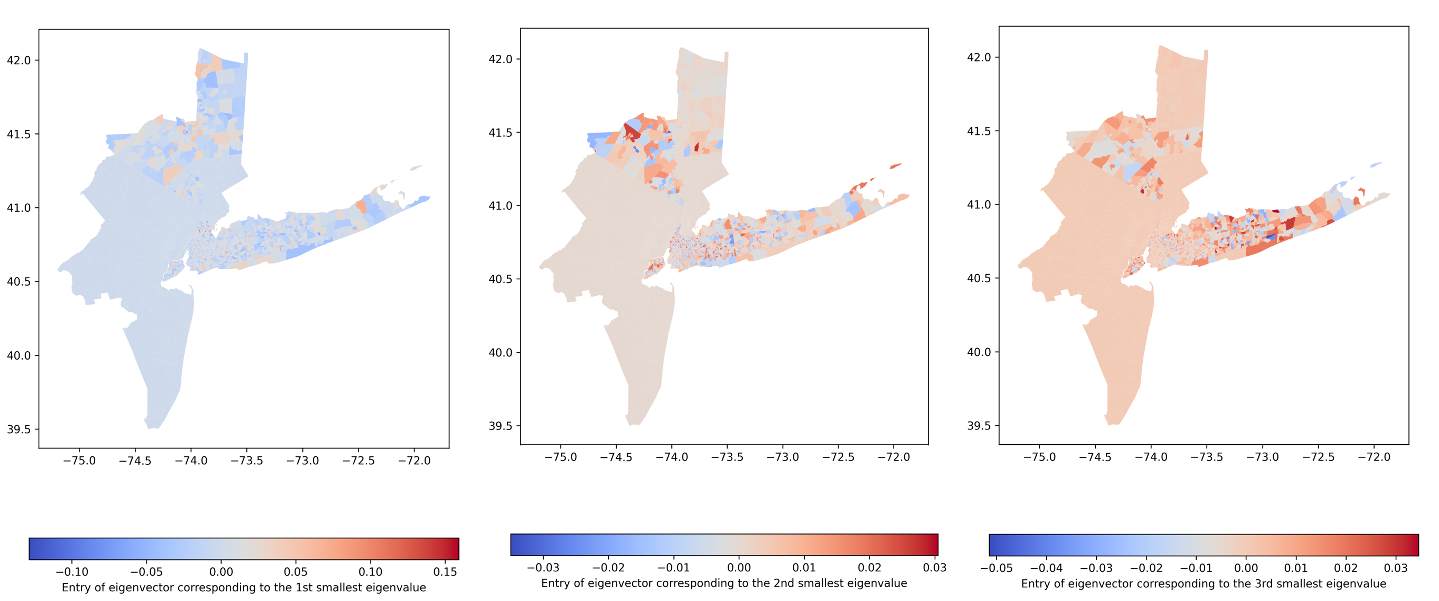
\includegraphics[width = 0.99\linewidth]{Figs/diffusionmap.png}
    \caption{扩散映射方法下,人口统计相关矩阵的前三小的正特征值对应的特征向量的空间分布。分别对应着纽约州的教育优势区域、贫困分布、和游客景点。}
    \label{fig:diffusionmap}
\end{figure}

Diffusion map是一种流形学习方法。其出发点在于:很多多元数据的数据元只能反映客体的一部分特征,只有将多个条目的survey合起来才能得到一个比较完整的刻画。提取多个条目的survey的“权重”并不是一件简单的事,因为很多时候数据的特征是非线性变化的。这种特征往往很难用一种全局度量来衡量。流形强调的是局部性质:流形(Manifold)是局部具有欧式空间性质的空间,包括各种纬度的曲线曲面,例如球体、弯曲的平面等。流形的局部和欧式空间是同构的。流形学习假设所处理的数据点分布在嵌入于外维欧式空间的一个潜在的流形体上,或者说这些数据点可以构成这样一个潜在的流形体。流形是线性子空间的一种非线性推广。以英国的普查数据为例:英国在每个区域统计两类人口统计学指标:关键指标和快速指标。总共有1450个特征。\cite{barter2019manifold},作者用布里斯托及其周边的3490个人口统计学单元作为主要研究对象。其中的分析找到了解释统计反馈的主要变量:大学生密度和贫困程度。

\subsection{稳定性:衡量城市交互系统对抗冲击的能力}

本研究借鉴了生态学的“稳定性”概念\cite{may1972will},拟提出一种衡量城市系统对抗外来冲击的指标,以判别流行病、谣言等外来因素在连通度日益提高的城市系统中是否会扩散开来。该框架的建立可以衡量城市系统的各个子系统的保守性,进而识别出城市中易于受攻击的子区域。该工作可以极大地取代多主体建模的复杂性,而得到同样鲁棒性的结果。

从概念上来讲,稳定性衡量一个系统各组成部分的平衡量由其相互作用形成的敏感程度,一直是大多数网络科学家关注的要点。由于缺乏足够的稳定性,城市流动网络这样的人类系统中经常无法幸免传染病和流言的爆发。这种性质通常是由于城市系统中过多的“节点”处于正反馈的网络路径上,进而难以规避。冲击扩散所留下的痕迹在缺乏稳定性的流动网络中积累。考虑到人类系统自发的稳定性缺失,我们研究:人类系统如何吸收外来的“冲击”?我们使用一个分析框架来量化人类系统自消化的稳定性,并给出了一个达到完全稳定的充分条件。最后,我们将城市内疫情爆发作为人类系统对外部冲击的不稳定诱导反应的案例进行研究,控制组件与自身的相互作用对于稳定疫情传播具有突出作用。因此,局部的保守性保证了人类系统的弹性,对它的监测增强了我们应对外部冲击的能力。

该工作的数学基础如下:介观尺度上,城市内部的人类移动性可以理解为场所$i = 1,2,\dots,n$之间的交互流,进而可以抽象成一个交互矩阵$W$, 其中矩阵$W$的元素$w_{i j}$代表场所$i$到场所$j$的流量。外来的冲击改变系统是由冲击系统的局部开始的,即各个场所受影响的人口$Y_1>0$, 而$Y_n = 0, n = 1,2,\dots, n$. 以流行病传播为例:某个场所出现了病例,病例进而随着交互流和局部扩散传播。疫情是否会扩散开,取决于患病子人口$(Y_1,\dots,Y_n)^T$在矩阵$W$作用下的稳定性:如果稳定性高,则疫情流行度会维持在$0$附近,即不会爆发;如果稳定性低,则疫情会以很高的概率爆发。鉴于不同的城市特征和流行病等冲击的不同,不同城市的交互流对外部冲击的反应非常异质。然而,从统计角度来看上看,城市系统的交互模式有几个共同的特征:首先,人们经常去人口密集或热门的地方,使得这类地方成为控制冲击的关键位置;其次,停留时间加权下,局部交互占总交互的比例对于不同的城市系统都保持在10-20\% 左右,但是,城市在面对疫情等冲击时,短距离的交互会因为补偿效应而占有更高的比例(如图\ref{fig:allee1}f)。这些人类流动的特征都会影响社会在面对外部冲击时的稳定性。基于以上的观察,我们建立了一个模型来解释外来冲击是如何随着人类流动而积累的。每个场所受冲击的人口数随时间的变化可以由下述方程确定:\begin{equation}
    \begin{split}
        \frac{d Y_n}{d t} = \alpha X_n (w_{nn} \theta Y_n / N_n + (1-\delta) \Delta F_n^I) - \beta Y_n, \\
        \text{其中}\quad \Delta F_n^I = \sum_{m \ne n} (w_{mn} Y_m / N_m - w_{nm} Y_n / N_n)
    \end{split}\label{eq:allee_basic}
\end{equation}是场所$n$受其他场所冲击的人口数,$\theta$和$\delta$分别代表了外在冲击影响下人类移动性在局部和全局的扩散系数。传播速度和遗忘速度则分别是$\alpha$和$\beta$. 利用一个疫情传播的易感-患病-移除(SIR)场景下的符号系统,我们将受冲击子人口的交互矩阵近似为\begin{equation}
    A^t_{m n}=\begin{cases}
\alpha(1-\delta)\left[ w_{m n} I_{m} / I_{n}N_{m} - w_{n m} / N_{n}\right] & m \neq n, \\
\theta \alpha S_{n}-\beta & m=n.
\end{cases}
\end{equation}最后,我们定义:\textbf{受冲击人口$Y$的交互矩阵$A$的负特征值的比例为外来冲击下,城市交互系统的稳定性。}\begin{figure}
    \centering
    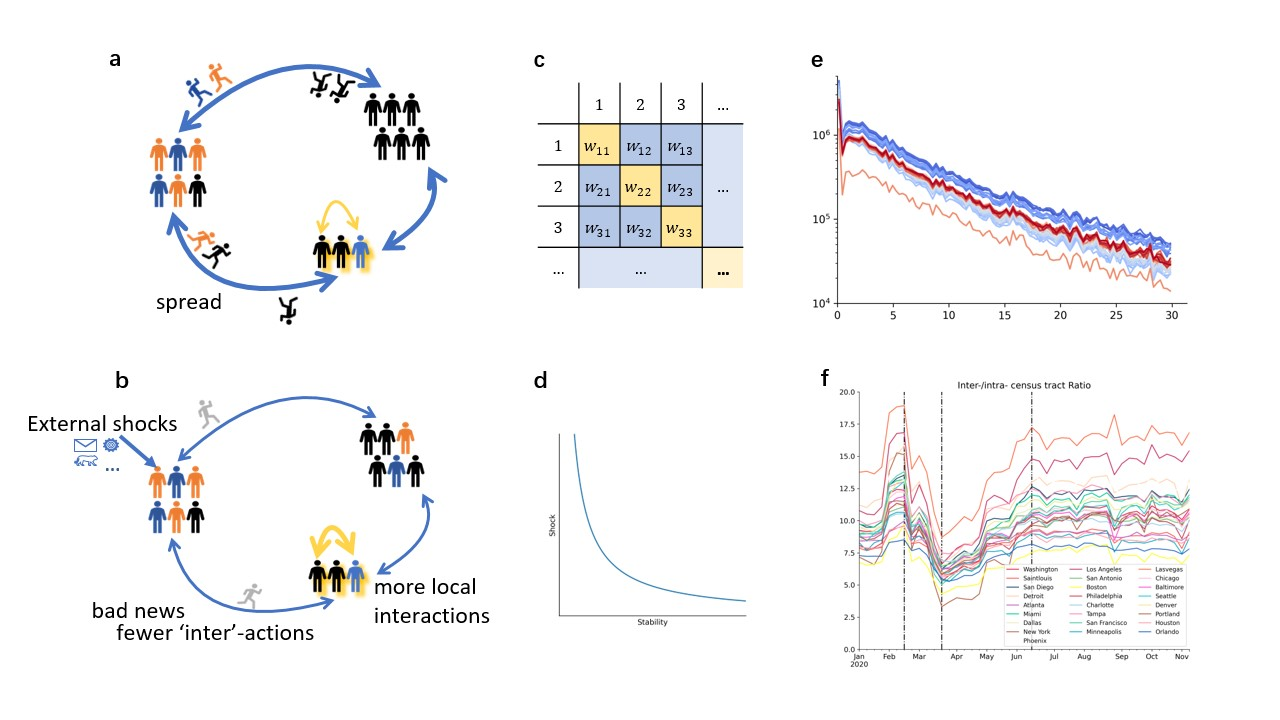
\includegraphics[width = 0.9\linewidth]{Figs/Figure1.jpg}
    \caption{\textbf{城市稳定性的框架图}。\textbf{a-b}, 人类系统(城市)面对外部冲击时的反应。冲击从一些元人口渗透到城市中,并通过经常性的流动网络和地方互动传播。\textbf{c}, 城市的抽象流动矩阵:在冲击期间,社区内部的访问更为频繁,对应$\theta > 1$. \textbf{d}, 系统的稳定性与其抵抗冲击转为爆发的能力之间的负向关系。 \textbf{e}, 华盛顿特区个体流动性的半径分布。最冷的颜色代表2020年的第一周,而最暖的颜色代表最新的。考虑到COVID-19的冲击,跨社区个体流动性的规模下降,恢复模式不变。\textbf{f},2020年1月至6月1日美国25个城市人口普查区间和人口普查区内流动意向的周比值。趋势代表了城市地区个别的运动半径,在2月中旬达到顶点,即左边的虚线,直到3月下旬才下降,即中间的虚线。这一结果支持了局部相互作用的作用在检疫期增加的说法。}
    \label{fig:allee1}
\end{figure}

\begin{figure}
    \centering
    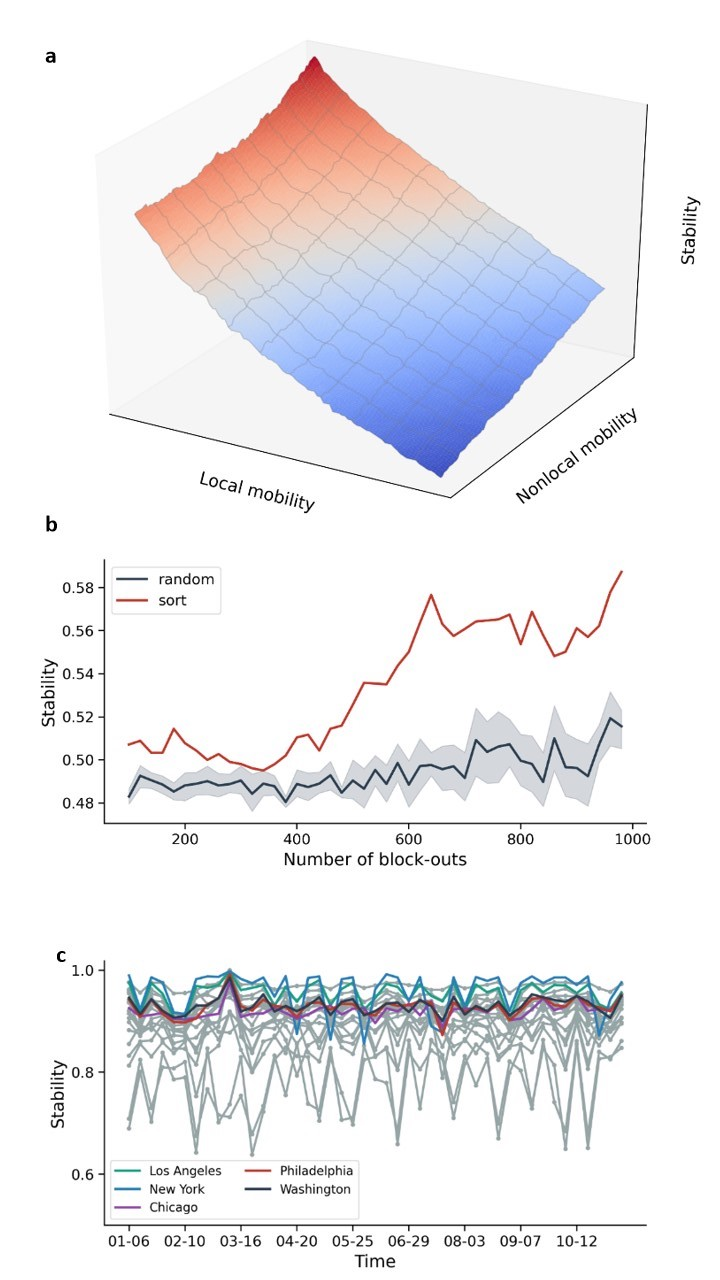
\includegraphics[width = 0.9\linewidth]{Figs/Figure2.jpg}
    \caption{\textbf{城市稳定性的框架图}。\textbf{a-b}, 人类系统(城市)面对外部冲击时的反应。冲击从一些元人口渗透到城市中,并通过经常性的流动网络和地方互动传播。\textbf{c}, 城市的抽象流动矩阵:在冲击期间,社区内部的访问更为频繁,对应$\theta > 1$. \textbf{d}, 系统的稳定性与其抵抗冲击转为爆发的能力之间的负向关系。 \textbf{e}, 华盛顿特区个体流动性的半径分布。最冷的颜色代表2020年的第一周,而最暖的颜色代表最新的。考虑到COVID-19的冲击,跨社区个体流动性的规模下降,恢复模式不变。\textbf{f},2020年1月至6月1日美国25个城市人口普查区间和人口普查区内流动意向的周比值。趋势代表了城市地区个别的运动半径,在2月中旬达到顶点,即左边的虚线,直到3月下旬才下降,即中间的虚线。这一结果支持了局部相互作用的作用在检疫期增加的说法。}
    \label{fig:allee1}
\end{figure}

\begin{figure}
    \centering
    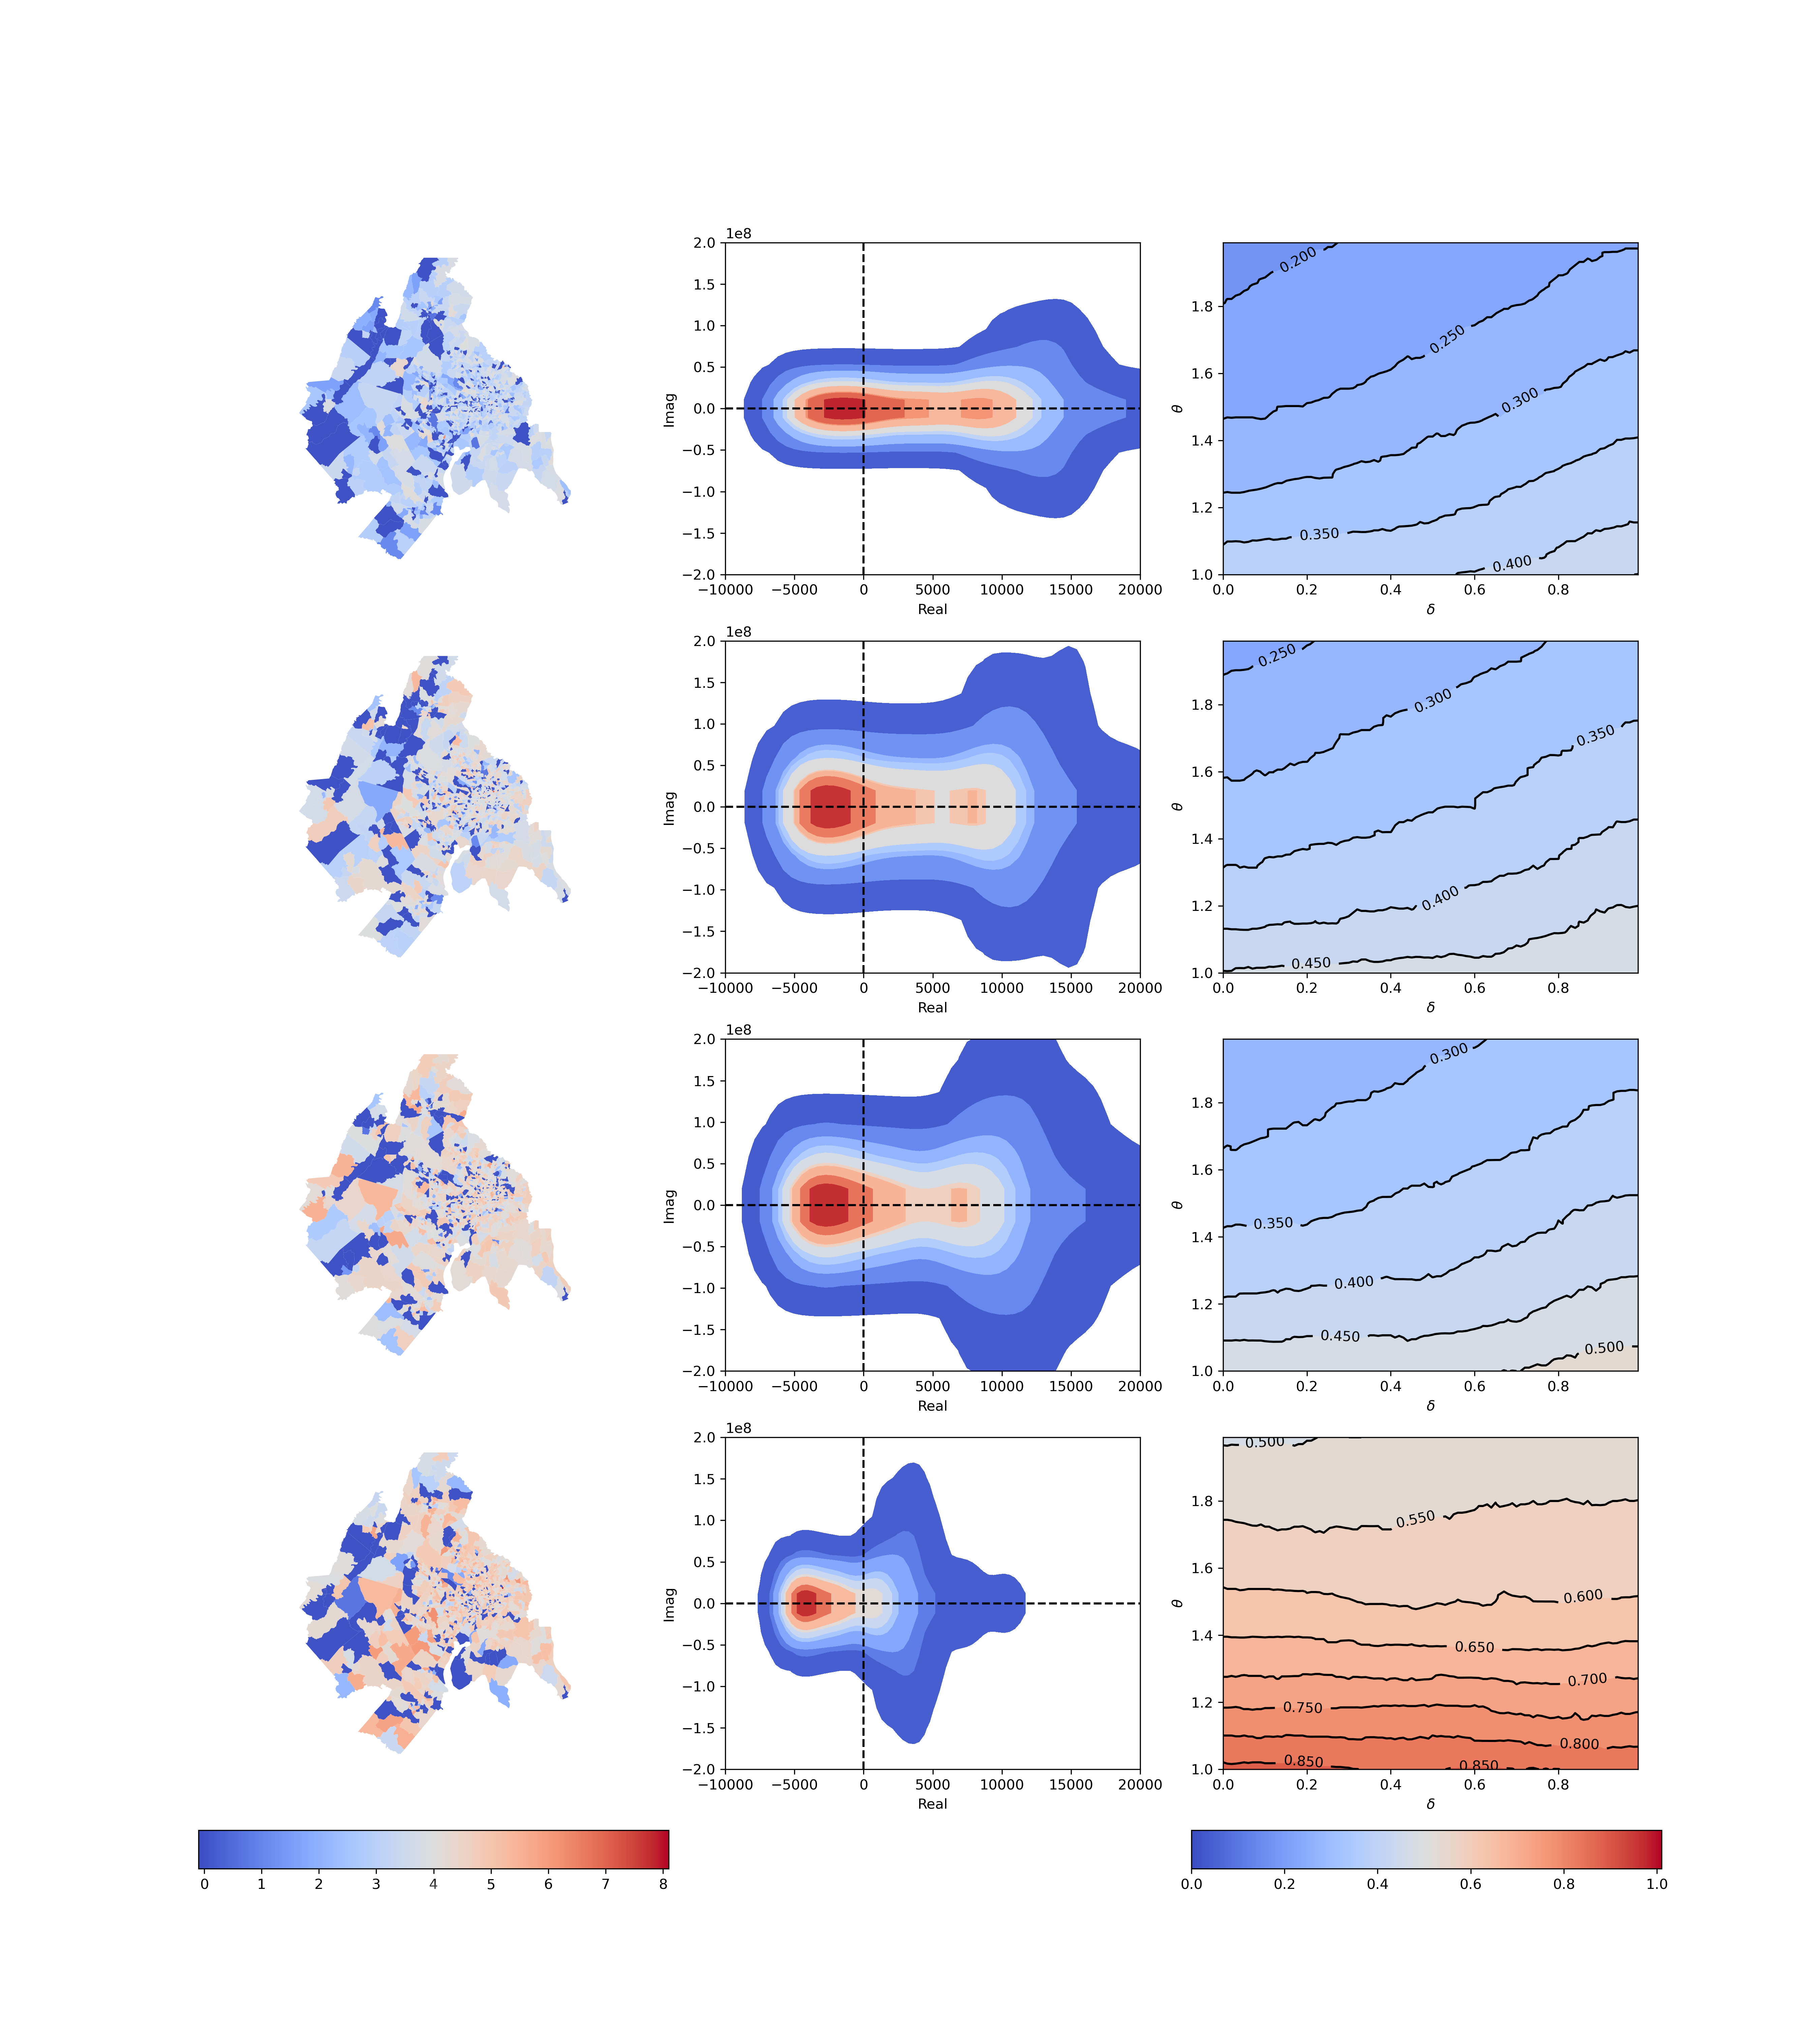
\includegraphics[width = 0.9\linewidth]{Figs/Figure3.png}
    \caption{\textbf{城市稳定性的框架图}。\textbf{a-b}, 人类系统(城市)面对外部冲击时的反应。冲击从一些元人口渗透到城市中,并通过经常性的流动网络和地方互动传播。\textbf{c}, 城市的抽象流动矩阵:在冲击期间,社区内部的访问更为频繁,对应$\theta > 1$. \textbf{d}, 系统的稳定性与其抵抗冲击转为爆发的能力之间的负向关系。 \textbf{e}, 华盛顿特区个体流动性的半径分布。最冷的颜色代表2020年的第一周,而最暖的颜色代表最新的。考虑到COVID-19的冲击,跨社区个体流动性的规模下降,恢复模式不变。\textbf{f},2020年1月至6月1日美国25个城市人口普查区间和人口普查区内流动意向的周比值。趋势代表了城市地区个别的运动半径,在2月中旬达到顶点,即左边的虚线,直到3月下旬才下降,即中间的虚线。这一结果支持了局部相互作用的作用在检疫期增加的说法。}
    \label{fig:allee1}
\end{figure}

\subsection{从众心理驱动下的介观模式形成问题}

城市中的多种传播过程背后都有着同样的数学机制\cite{gao2019effects, ribeiro2020city}。比如流行病、谣言、方言、城市功能分化、社区形成等。这一节中,我们以流行病传播为例,讨论传播过程如何在城市的介观层次上固定下来。

标准的疾病模型将流行病的复杂性降低为简单的过程,提供了有用的见解。把复杂的空间交互行为还原成个体对之间的交互的处理,可以概括为质量作用近似(mass-action approximation)上\cite{mollison1995epidemic}。这个假设考虑的是一个随机混合的人口,忽略了家庭结构、社会集会和不同个体的不同行为。因此,质量作用模型受到严重限制,因为它们只关注每个病例引起的平均感染数量,即基本传染数$R_0$ ,而忽略了潜在的异质性\cite{hebert2020beyond}。在依赖质量作用假设的情况下,设计有针对性的干预措施也存在概念问题。我们应该把干预措施的目标放在哪里,它们的影响应该是什么?我们通过引入高阶接触模式来解决这些问题。

流行病等传播过程进行的同时,心理因素也起到了重要作用。在疫苗尚未完全普及的现在,非药物干预(non-pharmaceutical interventions, NPSs)以及人们对其的态度有着决定性的地位。很多国家的早起宣传里,戴口罩是只有患者需要做的防疫措施。这使得社会形成戴口罩的共识变得异常困难\cite{lai2020effect, van2020face, Adolph2020PandemicPT, hellewell2020feasibility, Wolf2020AwarenessAA, Cheng2020TheRO, eikenberry2020to, erku2020fear, enberg2020covid}。这种误导或认识的时空差异有时甚至来自权威机构和研究者,他们对口罩供应缺失的强调所产生的对大众会产生心理影响\cite{biancovilli2020governments,landi2020should,sugaya2020real,weill2020social},并通过从众心理进一步传播。话语和顺应性使得社会对戴口罩难以达成共识,可能导致社会意识的分裂~\cite{holme2006nonequilibrium}。

理论上,通过统计物理学和心理学对促进健康关注的集体适应行为进行了广泛的研究~\cite{castellano2009statistical, centola2007complex, centola2010spread, centola2011experimental, christakis2007spread}。最核心的问题之一是,一个失衡的系统如何快速得到有序的发展。流行病的许多全球特征,如基本繁殖数,可能起源于社会群体的异质混合,对非药物干预的接受程度不同。比如戴口罩在被证明对COVID-19等呼吸道疾病有效,但对戴口罩的误导和歧视依然存在,这使得戴口罩的社会共识极难形成,反而加剧了社会关系的异质性。



在本信中,我们提出了一个异质性在不同行为群体和流行病之间传播的网络模型。我们假设个体选择戴口罩的变化是由顺应性驱动的,而流行病的传播则是通过研究良好的易感者-感染者-易感者(SIS)模型进行的。顺应性假设是合理的,因为类似健康行为的传播得到了实验验证~\cite{christakis2008collective, zhang2016support}。我们在各种接触网络上实现了这一点,并比较了分析平均场公式中的现象。在模型中,$N$代理通过联系网络中的链接连接。每个代理是否改变要么她是感染者,要么她是一个三角形中的少数人。我们研究了合成网络和现实世界的网络,它们对应于不同规模的相互作用。

\begin{figure}
    \centering
    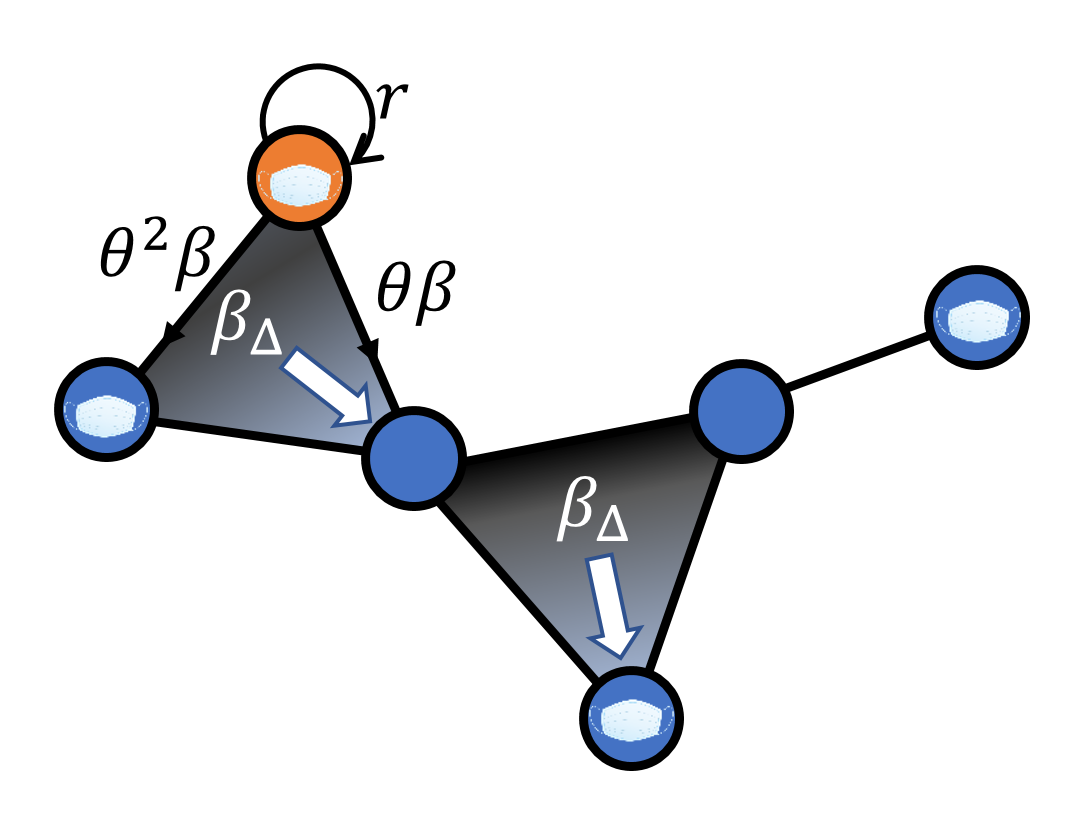
\includegraphics[width = 0.7\linewidth]{Figs/masksketch.png}
    \caption{意见与疾病共同演化模型。}
    \label{fig:masksketch}
\end{figure}



\section{预期创新点}

本文通过引入和构建较多的数学工具,对城市介观尺度下空间模式的提取、交互模式的性质、局部模式的涌现进行研究。本文的几个主要结果改进了地理大数据采集的设计,提出了定量衡量城市政策效果的方法,证明了介观尺度模式涌现的必然性。预期创新点如下:\begin{enumerate}
    \item 改进扩散映射方法,引入负相似性的概念,建立更广义的城市组件关联关系,挖掘了更多的诸如对偶结构、收缩城市结构等城市内蕴结构;
    \item 建立了城市稳定性的量化框架,以极快的运算效率衡量出城市面临疫情等外来冲击时的抵抗能力,以及各种时空尺度的政策在控制冲击。同时该框架亦可发现冲击扩散的关键节点。
    \item 通过考察一类较为通用的复杂网络动态及其
\end{enumerate}